
\documentclass[acmlarge,nonacm=true]{acmart}
\usepackage{adjustbox}
\usepackage{multirow}
\usepackage{graphicx}
\usepackage{afterpage}
\usepackage{subcaption}

\newcommand\blankpage{%
	\null
	\thispagestyle{empty}%
	\addtocounter{page}{-1}%
	\newpage}

%%
%% \BibTeX command to typeset BibTeX logo in the docs
\AtBeginDocument{%
  \providecommand\BibTeX{{%
    \normalfont B\kern-0.5em{\scshape i\kern-0.25em b}\kern-0.8em\TeX}}}


\begin{document}
	
	\begin{titlepage}
		\begin{center}
			\vspace*{1cm}
			
\includegraphics[width=0.7\textwidth]{fig/ntu_logo}
			\vspace{0.8cm}
			\linebreak
			\Huge
			\textbf{Experiment 5: Transformations and Motions}
			
			\vspace{0.5cm}
			\LARGE
			CZ2003 Computer Graphics and Visualization
			
			\vspace{1.5cm}
			\textbf{SS3}\\
			
			\begin{table}[h]
				\begin{tabular}{lc}
					Name & Matric Number \\\hline
					Pang Yu Shao & U17216\underline{\textbf{80}}D \\
				\end{tabular}
			\end{table}
			
			
			
			\vfill
			
			\vspace{0.8cm}
			
			
			
			\Large
			SCHOOL OF COMPUTER SCIENCE AND ENGINEERING\\
			NANYANG TECHNOLOGICAL UNIVERSITY\\
			SINGAPORE\\
			6th April 2021
			
		\end{center}
	\end{titlepage}

 

%%
%% The "title" command has an optional parameter,
%% allowing the author to define a "short title" to be used in page headers.
\title{CZ2003 Computer Graphics and Visualization}

%%
%% The "author" command and its associated commands are used to define
%% the authors and their affiliations.
%% Of note is the shared affiliation of the first two authors, and the
%% "authornote" and "authornotemark" commands
%% used to denote shared contribution to the research.


\author{Pang Yu Shao}
\email{C170134@e.ntu.edu.sg}
\affiliation{\institution{Nanyang Technological University}}

%%
%% By default, the full list of authors will be used in the page
%% headers. Often, this list is too long, and will overlap
%% other information printed in the page headers. This command allows
%% the author to define a more concise list
%% of authors' names for this purpose.
\renewcommand{\shortauthors}{Pang Yu Shao}






%%
%% This command processes the author and affiliation and title
%% information and builds the first part of the formatted document.

% \begin{teaserfigure}
% 	\includegraphics[width=\textwidth]{bccell}
% 	\caption{Breast Cancer Cell. Photograph by National Cancer Institute [Public domain], via Wikimedia
% 		Commons. (\url{https://w.wiki/kS3}).}
% 	\Description{A breast cancer cell seen through an electron microscope.}
% \end{teaserfigure}
% \maketitle



\tableofcontents
\newpage
\section{Transforming a Defined 3-D Curve}
\subsection{Deriving Transformation Matrix}
\label{section:1a}
First, a transformation matrix is defined for rotating by $\frac{\pi}{2}$ about an axis parallel to axis Y,
and passing through the point with coordinates $(M+5, 0, 0)$. Since M = 10, $(15, 0, 0)$.\\\\
Therefore to achieve this, first we align the axis with the Y-axis by translation of $(-15, 0, 0)$. Then, 
rotation of $\frac{\pi}{2}$ radians about axis Y is applied. Lastly, the initial translation is undone by 
applying a translation of $(15, 0, 0)$.\\\\
The three transformations can be defined using the following matrices:\\
$T_1 = \begin{bmatrix}
	1 & 0 & 0 & -15 \\
	0 & 1 & 0 & 0 \\
	0 & 0 & 1 & 0 \\
	0 & 0 & 0 & 1
 \end{bmatrix}$\\\\
$R = \begin{bmatrix}
	cos(\frac{\pi}{2}) & 0 & sin(\frac{\pi}{2}) & 0 \\
	0 & 1 & 0 & 0 \\
	-sin(\frac{\pi}{2}) & 0 & cos(\frac{\pi}{2}) & 0 \\
	0 & 0 & 0 & 1
 \end{bmatrix} = \begin{bmatrix}
	0 & 0 & 1 & 0 \\
	0 & 1 & 0 & 0 \\
	-1 & 0 & 0 & 0 \\
	0 & 0 & 0 & 1
 \end{bmatrix}$\\\\
$T_2 = \begin{bmatrix}
	1 & 0 & 0 & 15 \\
	0 & 1 & 0 & 0 \\
	0 & 0 & 1 & 0 \\
	0 & 0 & 0 & 1
 \end{bmatrix}$\\\\
The final transformation matrix, M can then be obtained:\\
$M = T_2 \cdot R \cdot T_1$\\\\
$M = \begin{bmatrix}
	1 & 0 & 0 & 15 \\
	0 & 1 & 0 & 0 \\
	0 & 0 & 1 & 0 \\
	0 & 0 & 0 & 1
 \end{bmatrix} \begin{bmatrix}
	0 & 0 & 1 & 0 \\
	0 & 1 & 0 & 0 \\
	-1 & 0 & 0 & 0 \\
	0 & 0 & 0 & 1
 \end{bmatrix}\begin{bmatrix}
	1 & 0 & 0 & -15 \\
	0 & 1 & 0 & 0 \\
	0 & 0 & 1 & 0 \\
	0 & 0 & 0 & 1
 \end{bmatrix}$\\\\
 $\ = \begin{bmatrix}
	1 & 0 & 0 & 15 \\
	0 & 1 & 0 & 0 \\
	0 & 0 & 1 & 0 \\
	0 & 0 & 0 & 1
 \end{bmatrix} \begin{bmatrix}
	0 & 0 & 1 & 0 \\
	0 & 1 & 0 & 0 \\
	-1 & 0 & 0 & 15 \\
	0 & 0 & 0 & 1
 \end{bmatrix}$\\\\
 $\ = \begin{bmatrix}
	0 & 0 & 1 & 15 \\
	0 & 1 & 0 & 0 \\
	-1 & 0 & 1 & 15 \\
	0 & 0 & 0 & 1
 \end{bmatrix}$\\\\
\newpage
\subsection{Applying Transformation Matrix to Parametrically Defined Curve}
The matrix obtained from section \ref{section:1a} is to be applied to the parametric
equations of the curve defined in experiment 1, exercise 3.
The following parametric functions defined the abovementioned curve.
\begin{displaymath}
	\mathbf{x_0(u) =  (8 - 15cos(2\pi u))cos(2\pi u)}
\end{displaymath}
\begin{displaymath}
	\mathbf{y_0(u) =  (8 - 15cos(2\pi u))sin(2\pi u)}
\end{displaymath}
\begin{displaymath}
	\mathbf{z_0(u) =  0}, 	u \in [0, 1]
\end{displaymath}
To obtain the transformed parametric equations, matrix multiplication can be used:\\

\begin{displaymath}
	\begin{bmatrix}
		x(u) \\
		y(u) \\
		z(u) \\
		1
	 \end{bmatrix} = \begin{bmatrix}
		0 & 0 & 1 & 15 \\
		0 & 1 & 0 & 0 \\
		-1 & 0 & 1 & 15 \\
		0 & 0 & 0 & 1
	 \end{bmatrix} \cdot \begin{bmatrix}
		x_0(u) \\
		y_0(u) \\
		z_0(u) \\
		1
	 \end{bmatrix}
\end{displaymath}

Therefore,
\begin{displaymath}
	x(u) =  z_0(u) + 15
\end{displaymath}
\begin{displaymath}
	y(u) =  y_0(u)
\end{displaymath}
\begin{displaymath}
	z(u) =  -x_0(u) + z_0(u) + 15
\end{displaymath}\\
\begin{displaymath}
	\mathbf{x(u) = 15}
\end{displaymath}
\begin{displaymath}
	\mathbf{y(u) =  (8 - 15cos(2\pi u))sin(2\pi u)}
\end{displaymath}
\begin{displaymath}
	\mathbf{z(u) =  15 - (8 - 15cos(2\pi u))cos(2\pi u)}
\end{displaymath}
\begin{displaymath}
	u \in [0, 1]
\end{displaymath}
\\
By plotting the parametric equations defined above, we get the following images:

\begin{figure}[H]
	\begin{subfigure}{.33\textwidth}
		\centering
		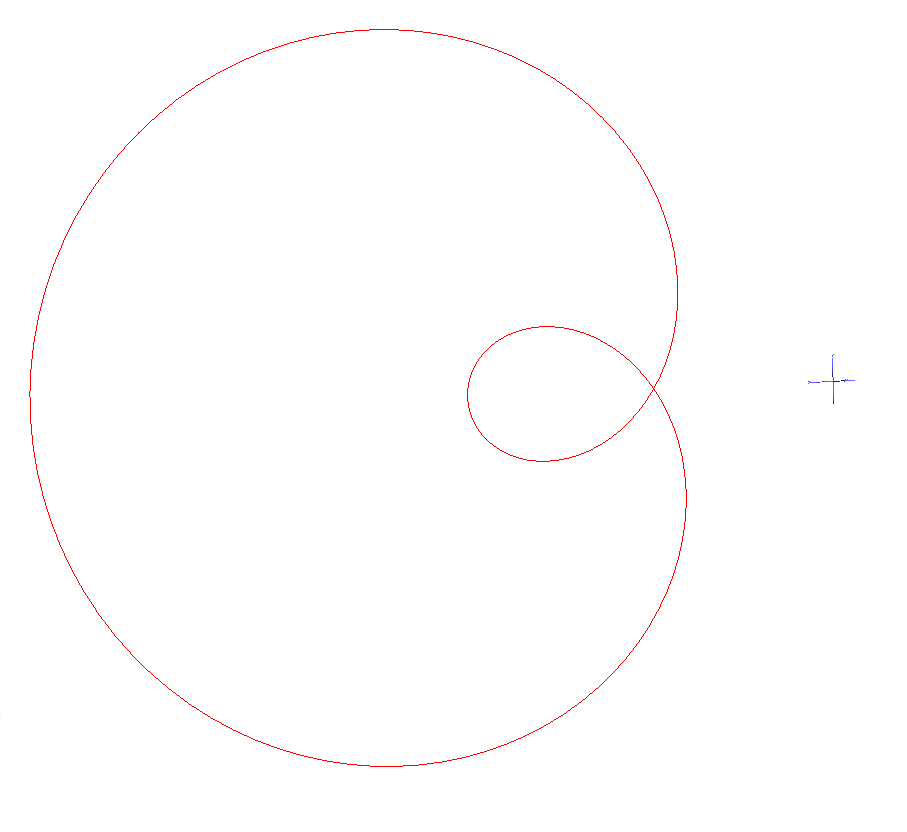
\includegraphics[width=.8\linewidth]{fig/1b_150}
		\caption{Resolution: 150}
	\end{subfigure}%
	\begin{subfigure}{.33\textwidth}
		\centering
		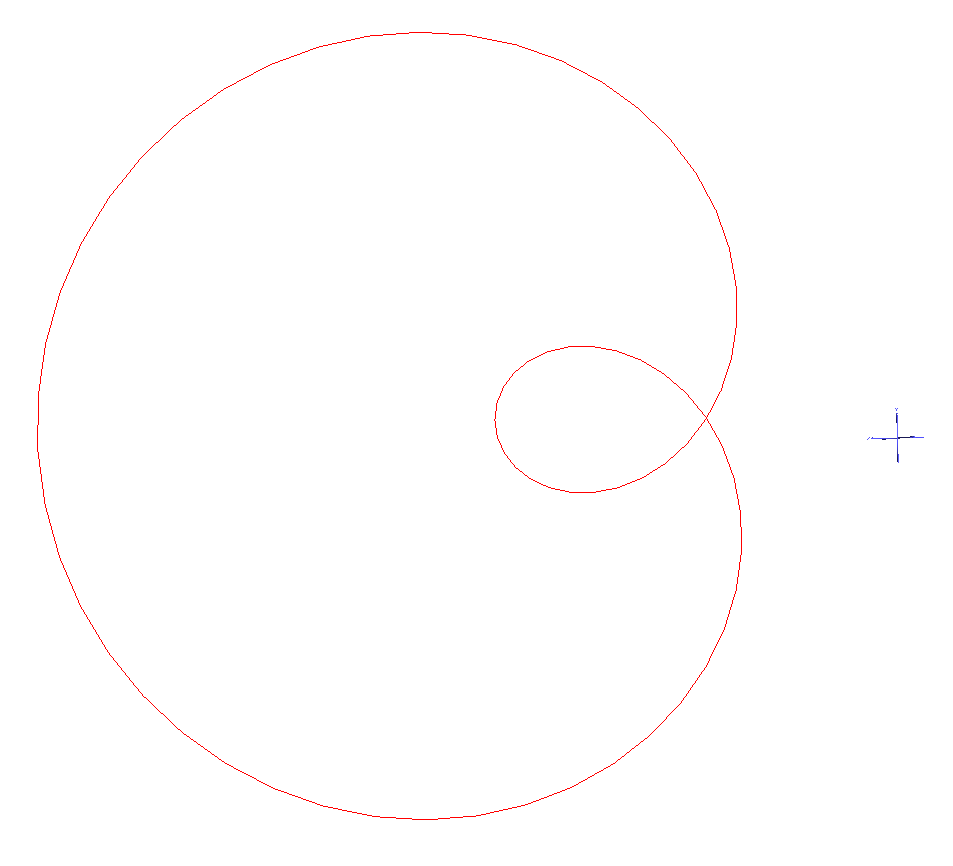
\includegraphics[width=.8\linewidth]{fig/1b_75}
		\caption{Resolution: 75}
	\end{subfigure}
	\begin{subfigure}{.33\textwidth}
			\centering
			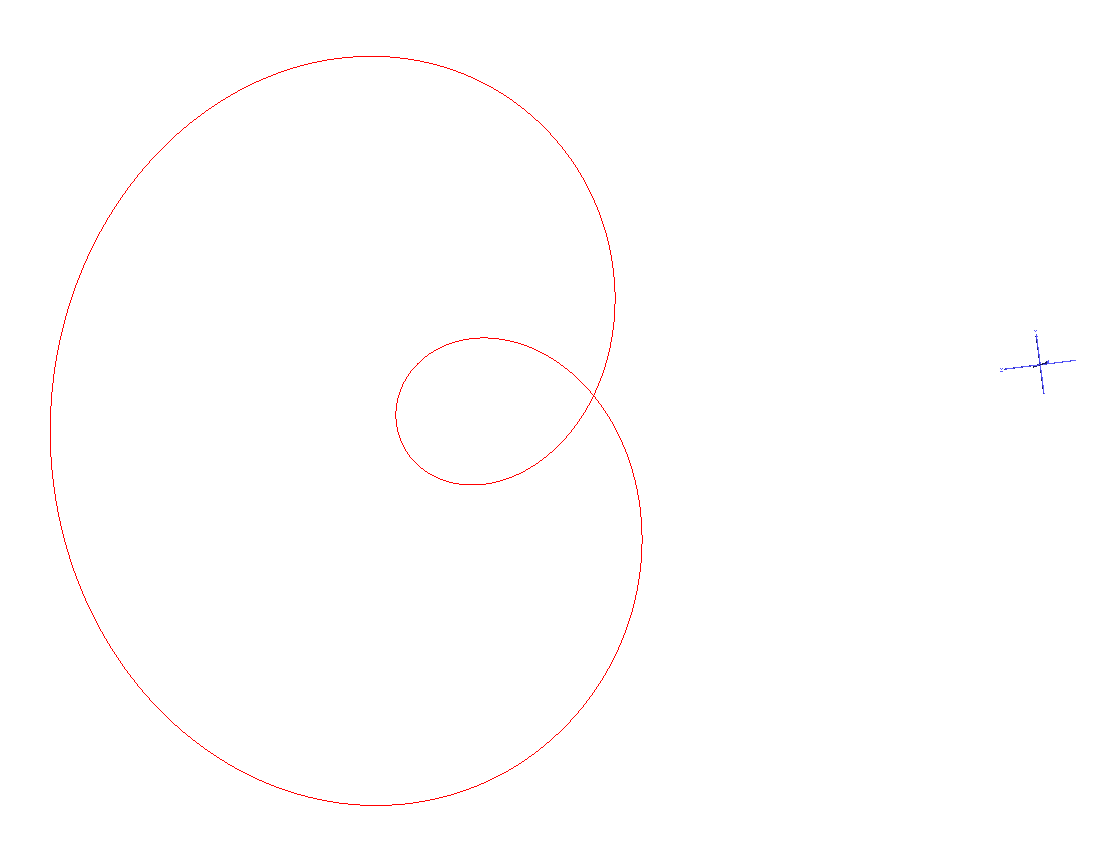
\includegraphics[width=.8\linewidth]{fig/1b_300}
			\caption{Resolution: 300}
	\end{subfigure}
	\caption{Plots of the parametrically defined curve in "\textbf{1b.wrl}" with differing resolutions}
	\label{fig:1b}
\end{figure}
As seen in Fig. \ref{fig:1b} above, a sampling resolution of \textbf{150} is the optimal 
resolution for rendering the curve. When the resolution is reduced to 75, the polyline interpolations can 
be seen when zoomed in. When the resolution is increased to 300, there is no visible difference 
in the rendered curve when compared to that rendered with resolution of 150.

\newpage
\section{Animating Transformation Motion with Deceleration}
By modfying the parametric definitions to include the time parameter, $t$,
The rotation can be animated with the following definitions:\\\\
\begin{displaymath}
	x(u,t) =  (1-\tau(t))*x_0(u) + \tau(t)*x_1(u)
\end{displaymath}
\begin{displaymath}
	y(u,t) =  (1-\tau(t))*y_0(u) + \tau(t)*y_1(u)
\end{displaymath}
\begin{displaymath}
	z(u,t) =  (1-\tau(t))*z_0(u) + \tau(t)*z_1(u)
\end{displaymath}\\
Since $y_0(u) = y_1(u)$,\\
\begin{displaymath}
	x(u,t) =  ((1-\tau(t))(8 - 15cos(2\pi u))cos(2\pi u)) + (15\tau(t))
\end{displaymath}
\begin{displaymath}
	y(u,t) =  (8 - 15cos(2\pi u))sin(2\pi u)
\end{displaymath}
\begin{displaymath}
	z(u,t) =  \tau(t)(15 - (8 - 15cos(2\pi u))cos(2\pi u))
\end{displaymath}
Lastly, the function to control the speed of animation (eceleration) is defined:\\
\begin{displaymath}
	\tau(t) =  sin(\frac{\pi}{2} \frac{t-t_1}{t_2-t_1})
\end{displaymath}
Since $t_1 = 0$ and $t_2 = 1$,
\begin{displaymath}
	\tau(t) =  sin(\frac{\pi}{2}t)
\end{displaymath}

The defined functions were then animated using ShapeExplorer, with the resolution set to \textbf{150}
since the shape is unchanged. The CycleInterval parameter is also set to \textbf{5} 
seconds. The curve can be seen to rotate from the X-Y plane until it is parallel with the Y-Z plane. 
The figure below shows the animation of the rotation.

\begin{figure}[H]
	\begin{subfigure}{.33\textwidth}
	  \centering
	  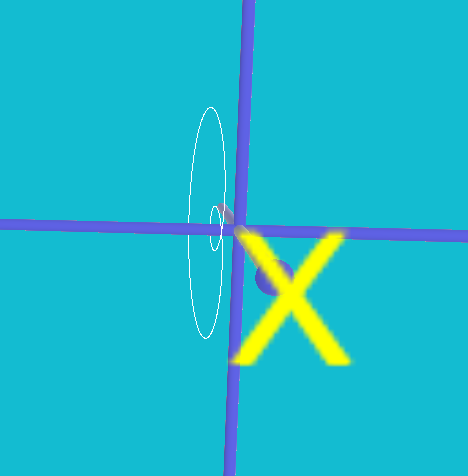
\includegraphics[width=.8\linewidth]{fig/2_start}
	  \caption{Start}
	\end{subfigure}%
	\begin{subfigure}{.33\textwidth}
	  \centering
	  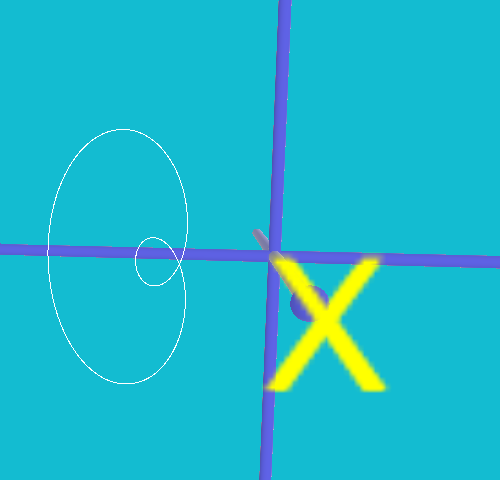
\includegraphics[width=.8\linewidth]{fig/2_mid}
	  \caption{Middle}
	\end{subfigure}
	\begin{subfigure}{.33\textwidth}
		\centering
		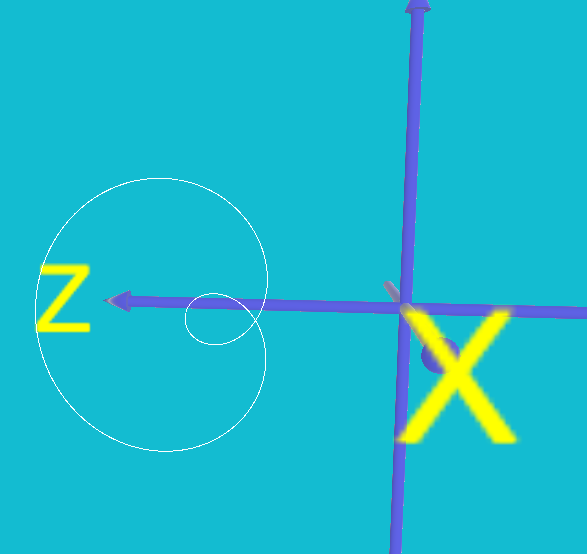
\includegraphics[width=.8\linewidth]{fig/2_end}
		\caption{End}
	  \end{subfigure}
	\caption{Frames of the animation defined in "\textbf{2.Func}" at different stages}
	\label{fig:2}
\end{figure}


\pagebreak

\section{Morphing Between Two Surfaces}
\subsection{Converting and Displaying Surfaces}
\subsubsection{Surface 10 (M)} From Table 3, Surface 10 is defined as:\\
$x = 0.5((\phi-0.5sin(\phi))-3)$\\
$y = 0.5cos(4\alpha\pi)(1-0.5cos(\phi))$\\
$z = 0.5sin(4\alpha\pi)(1-0.5cos(\phi))$\\
$0\leq\alpha\leq0.5,\ 0\leq\phi\leq2\pi$\\\\
Therefore, they can be convered into the following parametric functions:\\
$x(u,v) = 0.5((2\pi u-0.5sin(2\pi u))-3)$\\
$y(u,v) = 0.5cos(2\pi v)(1-0.5cos(2\pi u))$\\
$z(u,v) = 0.5sin(2\pi v)(1-0.5cos(2\pi u))$\\
$u,v \in [0,1]$\\\\
By entering the above functions onto ShapeExplorer, the following curves are rendered:\\
\begin{figure}[H]
	\begin{subfigure}{.33\textwidth}
		\centering
		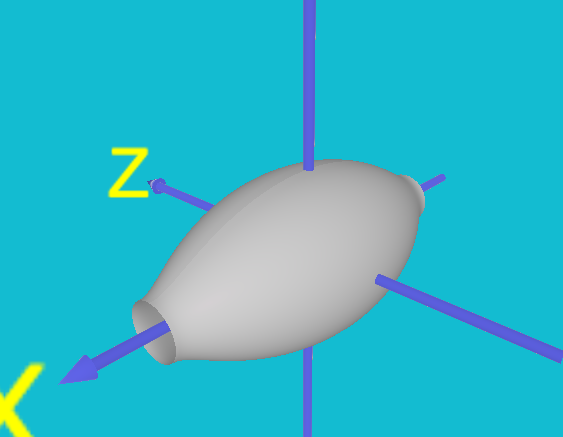
\includegraphics[width=.8\linewidth]{fig/3ai_50_50.PNG}
		\caption{Resolution: 50 50}
	\end{subfigure}%
	\begin{subfigure}{.33\textwidth}
		\centering
		
\includegraphics[width=.8\linewidth]{fig/3ai_25_25.PNG}
		\caption{Resolution: 25 25}
	\end{subfigure}
	\begin{subfigure}{.33\textwidth}
			\centering
			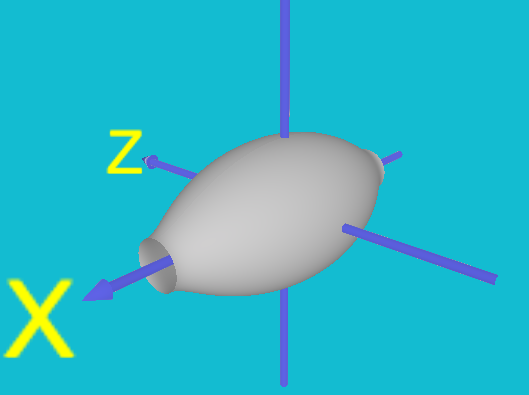
\includegraphics[width=.8\linewidth]{fig/3ai_100_100.PNG}
			\caption{Resolution: 100 100}
	\end{subfigure}
	\caption{Plots of the parametrically defined surface in "\textbf{3a1.Func}" with differing resolutions}
	\label{fig:3a1}
\end{figure}

As seen in Fig. \ref{fig:3a1} above, a sampling resolution of \textbf{50} for u and v is the optimal 
resolution for rendering the surface. When the resolution is reduced to 25, the surface is not smooth
when zoomed in and the interpolations can be seen. When the resolution is increased to 100, there is no visible difference 
in the rendered surface when compared to that rendered with resolution of 50.

\newpage
\subsubsection{Surface 18 (N+M)} From Table 3, Surface 18 is defined as:\\
$x = (cos(0.25\theta) + 1)cos(\phi)$\\
$y = sin(0.25\theta)cos(\phi)$\\
$z = sin(\phi)$\\
$0\leq\theta\leq8\pi,\ 0\leq\phi\leq2\pi$\\\\
Therefore, they can be convered into the following parametric functions:\\
$x(u,v) = (cos(2\pi u) + 1)cos(2\pi v)$\\
$y(u,v) = sin(2\pi u)cos(2\pi v)$\\
$z(u,v) = sin(2\pi v)$\\
$u,v\in[0,1]$\\\\
By entering the above functions onto ShapeExplorer, the following curves are rendered:\\
\begin{figure}[H]
	\begin{subfigure}{.33\textwidth}
		\centering
		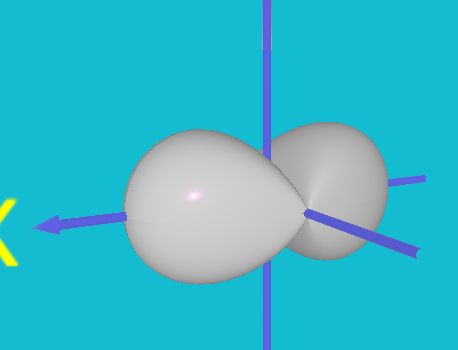
\includegraphics[width=.8\linewidth]{fig/3aii_50_50.PNG}
		\caption{Resolution: 50 50}
	\end{subfigure}%
	\begin{subfigure}{.33\textwidth}
		\centering
		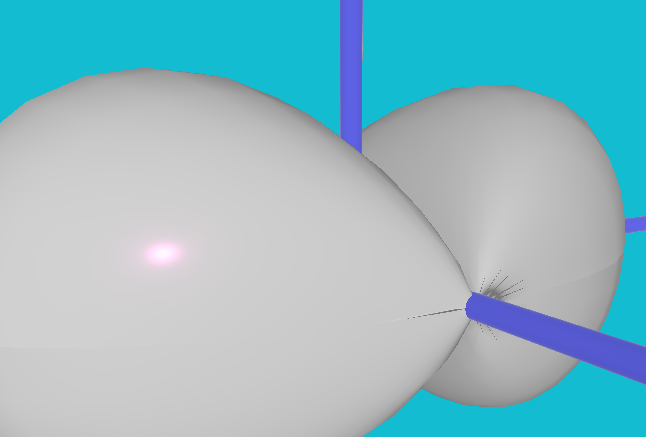
\includegraphics[width=.8\linewidth]{fig/3aii_25_25.PNG}
		\caption{Resolution: 25 25}
	\end{subfigure}
	\begin{subfigure}{.33\textwidth}
			\centering
			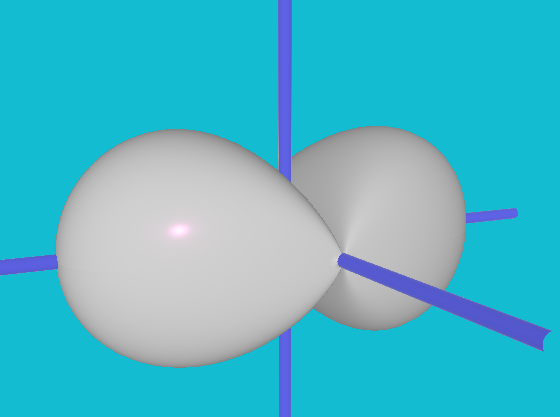
\includegraphics[width=.8\linewidth]{fig/3aii_100_100.PNG}
			\caption{Resolution: 100 100}
	\end{subfigure}
	\caption{Plots of the parametrically defined surface in "\textbf{3a2.Func}" with differing resolutions}
	\label{fig:3a2}
\end{figure}

As seen in Fig. \ref{fig:3a2} above, a sampling resolution of \textbf{50} for u and v is the optimal 
resolution for rendering the surface. When the resolution is reduced to 25, the surface is not smooth
when zoomed in and the interpolations can be seen. When the resolution is increased to 100, there is no visible difference 
in the rendered surface when compared to that rendered with resolution of 50.

\newpage
\subsection{Morphing Between Two Defined Surfaces}
From the above section, we obtained the following functions:\\
\textbf{Surface 10:}\\
$x_0(u,v) = 0.5((2\pi u-0.5sin(2\pi u))-3)$\\
$y_0(u,v) = 0.5cos(2\pi v)(1-0.5cos(2\pi u))$\\
$z_0(u,v) = 0.5sin(2\pi v)(1-0.5cos(2\pi u))$\\
$u,v \in [0,1]$\\\\
\textbf{Surface 18:}\\
$x_1(u,v) = (cos(2\pi u) + 1)cos(2\pi v)$\\
$y_1(u,v) = sin(2\pi u)cos(2\pi v)$\\
$z_1(u,v) = sin(2\pi v)$\\
$u,v\in[0,1]$\\\\
Since the morphing animation is back and forth, the speed control function
can be defined parametrically by:\\
$\tau(t) = 1 - |1 - 2t|$\\\\
Therefore, the morphing can be defined parametrically as:\\
$x(u,v,t) = x_0(u,v) + (x_1(u,v) - x_0(u,v))\tau(t)$\\
$y(u,v,t) = y_0(u,v) + (y_1(u,v) - y_0(u,v))\tau(t)$\\
$z(u,v,t) = z_0(u,v) + (z_1(u,v) - z_0(u,v))\tau(t)$\\
$u,v\in[0,1]$\\\\
The morphing animation is rendered using ShapeExplorer with a resolution of \textbf{50}
for both u and v as it is the optimal resolution found for both surfaces in the experiments
carried out in the previous sections. The CycleInterval parameter is also set to \textbf{5} 
seconds. The figure below shows the animation of the rotation.


\begin{figure}[H]
	\begin{subfigure}{.33\textwidth}
	  \centering
	  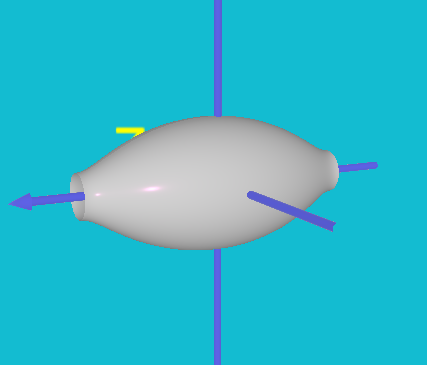
\includegraphics[width=.8\linewidth]{fig/3b_start}
	  \caption{Surface 10}
	\end{subfigure}%
	\begin{subfigure}{.33\textwidth}
	  \centering
	  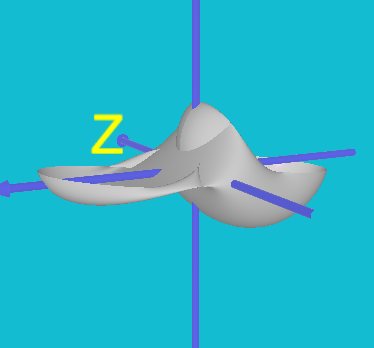
\includegraphics[width=.8\linewidth]{fig/3b_mid}
	  \caption{In-between}
	\end{subfigure}
	\begin{subfigure}{.33\textwidth}
		\centering
		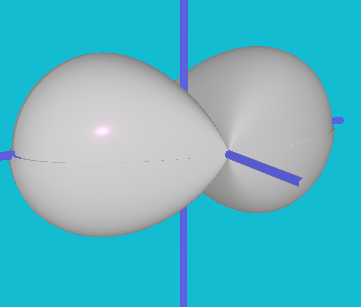
\includegraphics[width=.8\linewidth]{fig/3b_end}
		\caption{Surface 18}
	  \end{subfigure}
	\caption{Frames of the animation defined in "\textbf{3b.Func}" at different stages}
	\label{fig:2}
\end{figure}

Once the surface is morphed from surface 10 to surface 18, it morphs back to surface 10 as the 
speed control is defined to be uniform with back and forth effect.

\bibliographystyle{ACM-Reference-Format}
\newpage






\end{document}
\endinput
%%
%% End of file `sample-acmlarge.tex'.
